% $Id: NUOPC_implnotes.tex,v 1.3 2011/04/28 22:47:20 theurich Exp $

The NUOPC Layer is implemented in Fortran on top of the public ESMF Fortran API.

The NUOPC utility routines form a very straight forward Fortran API. The interface is defined using only native Fortran types and ESMF derived types. In order to access the NUOPC Layer utility API user code must include the following two {\tt use} lines:

\begin{verbatim}
  use ESMF_Mod
  use NUOPC
\end{verbatim}

The NUOPC generic components are implemented as a collection of Fortran modules. Each module implements a single, well specified set of standard {\tt ESMF\_GridComp} or {\tt ESMF\_CplComp} methods. The nomenclature of the generic component modules starts with the {\tt NUOPC\_} prefix, then continues with {\tt Driver}, {\tt Model}, {\tt Mediator}, or {\tt Connector} followed optionally by a string of descriptive terms.

The user code accesses the desired generic component(s) by including a {\tt use} line for each one. Each generic component defines a small set of public names that are made available to the user code through the {\tt use} statement. At a minimum the {\tt SetServices} method is made public. Some generic components also define a public internal state type by the standard name {\tt InternalState}. It is recommended that the following syntax is used when accessing a generic component (here with internal state):

\begin{verbatim}
  use NUOPC_DriverXYZ, only: &
    DriverXYZ_SS => SetServices, &
    DriverXYZ_IS => InternalState
\end{verbatim}

A generic component is used by user code to implement a specialized version of the component. The user code therefore also must implement a public {\tt SetServices} routine. The first thing this routine must do is call into the {\tt SetServices} routine provided by the generic component. It is through this step that the specialized component {\em inherits} from the generic component.

There are three mechanisms through which user code specializes generic components.

\begin{enumerate}

\item The specializing user code must set entry points for standard component methods not implemented by the generic component. Methods (and phases) that need to be implemented are clearly documented in the generic component description. The user code may further overwrite standard methods already implemented by the generic component code. However, this should rarely be necessary, and indicates that there may be a better fitting generic component available. Setting entry points for standard component methods is done in the {\tt SetServices} routine right after calling into the generic {\tt SetServices} method.

\item Some generic components require that specific methods are attached to the component. If a generic component uses specialization by attachable methods it will clearly document the specific method labels, i.e. the names by which these methods are registered, and what these methods are expected to implement. In some cases attachable methods can be optional. This is clearly documented. Attaching methods to the component should be done in the {\tt SetServices} routine right after setting entry points for standard component methods.

\item Some generic components provide access to an internal state type. The documentation of a generic component indicates which internal state members are used for specialization, and how they are expected to be set. Setting internal state members often requires the availability of other pieces of information. It may happend in the {\tt SetServices} routine, but more often inside a specialized standard entry point or an attachable method.

\end{enumerate}

Figure \ref{fig:NUOPCGenericComp} depicts the class structure of the NUOPC Generic Components. There are two trees, one is rooted in {\tt ESMF\_GridComp}, while the other is rooted in {\tt ESMF\_CplComp}.
\begin{figure}
\begin{center}
\scalebox{0.6}{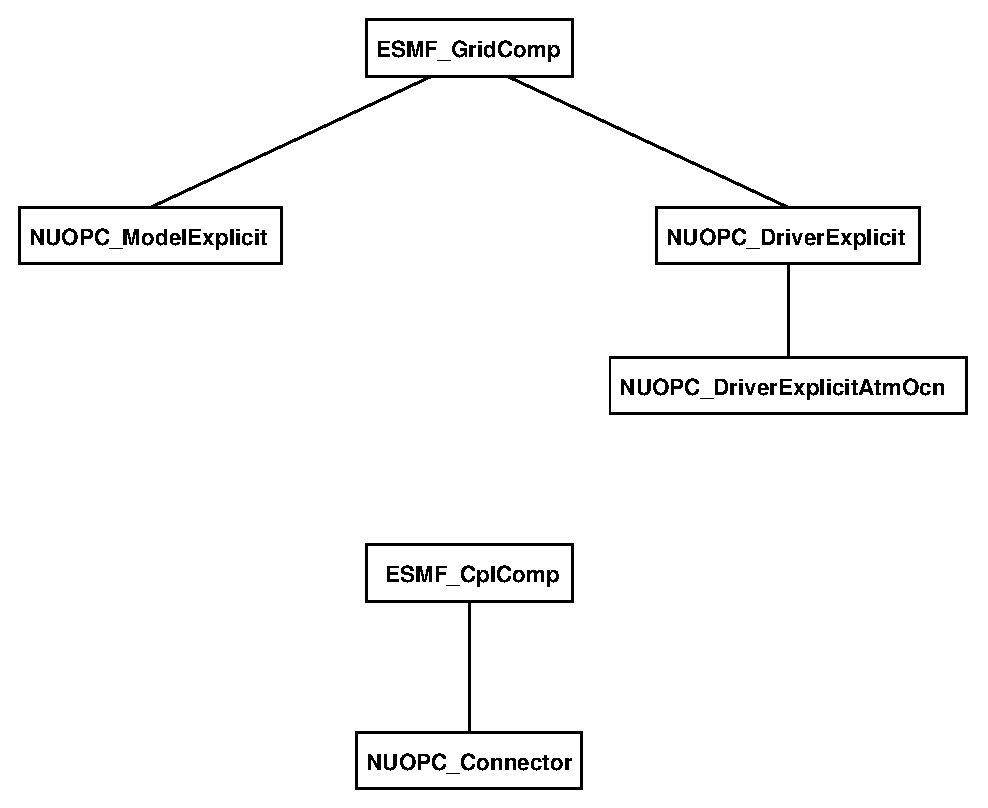
\includegraphics{NUOPC_GC}}
\end{center}
\caption{NUOPC Generic Component class structure.}
\label{fig:NUOPCGenericComp}
\end{figure}


